%\subsection*{Anhang}
%\label{anhang}
%TODO: Anhang Fixen


\begin{figure}[htb]
    \centering
    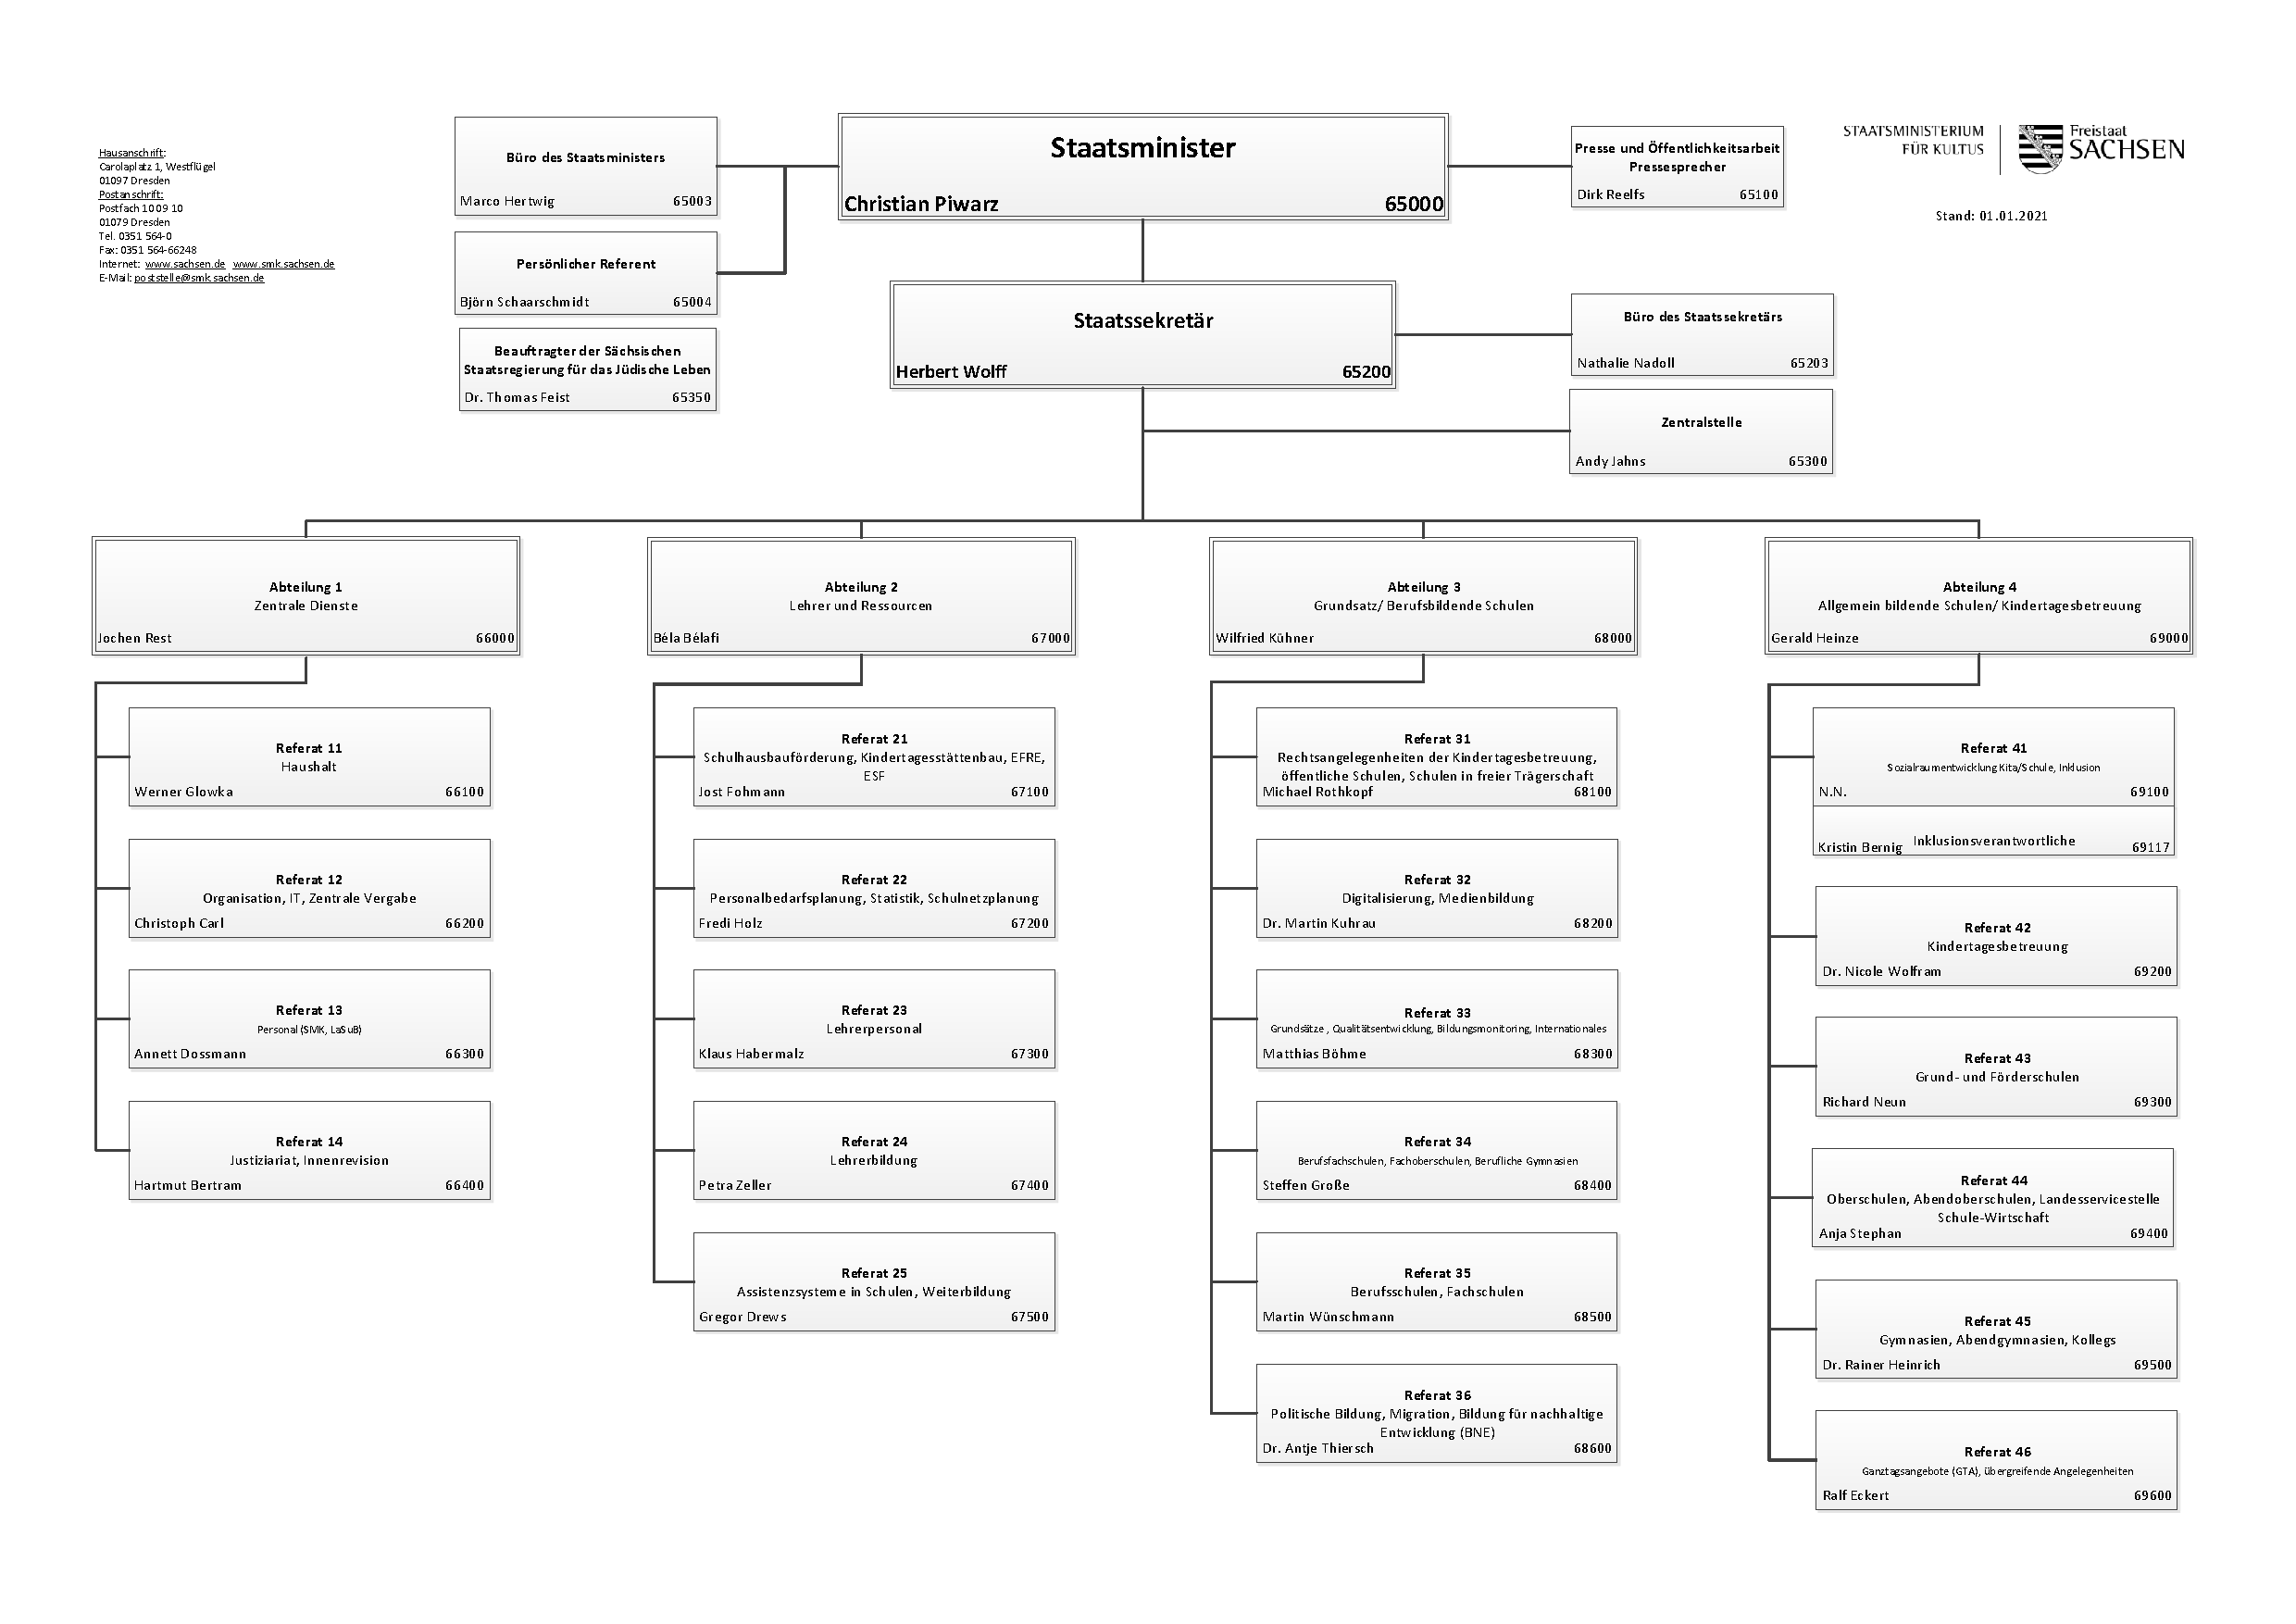
\includegraphics[angle=90, page=1,height=0.90\textheight, keepaspectratio]{anhang/abb/21_01_06_Organigramm_SMK.pdf}
    \caption[Organigramm des SMK]{Organigramm}
    \label{abb:Organigramm}
\end{figure}

\begin{figure}[htb]
    \centering
    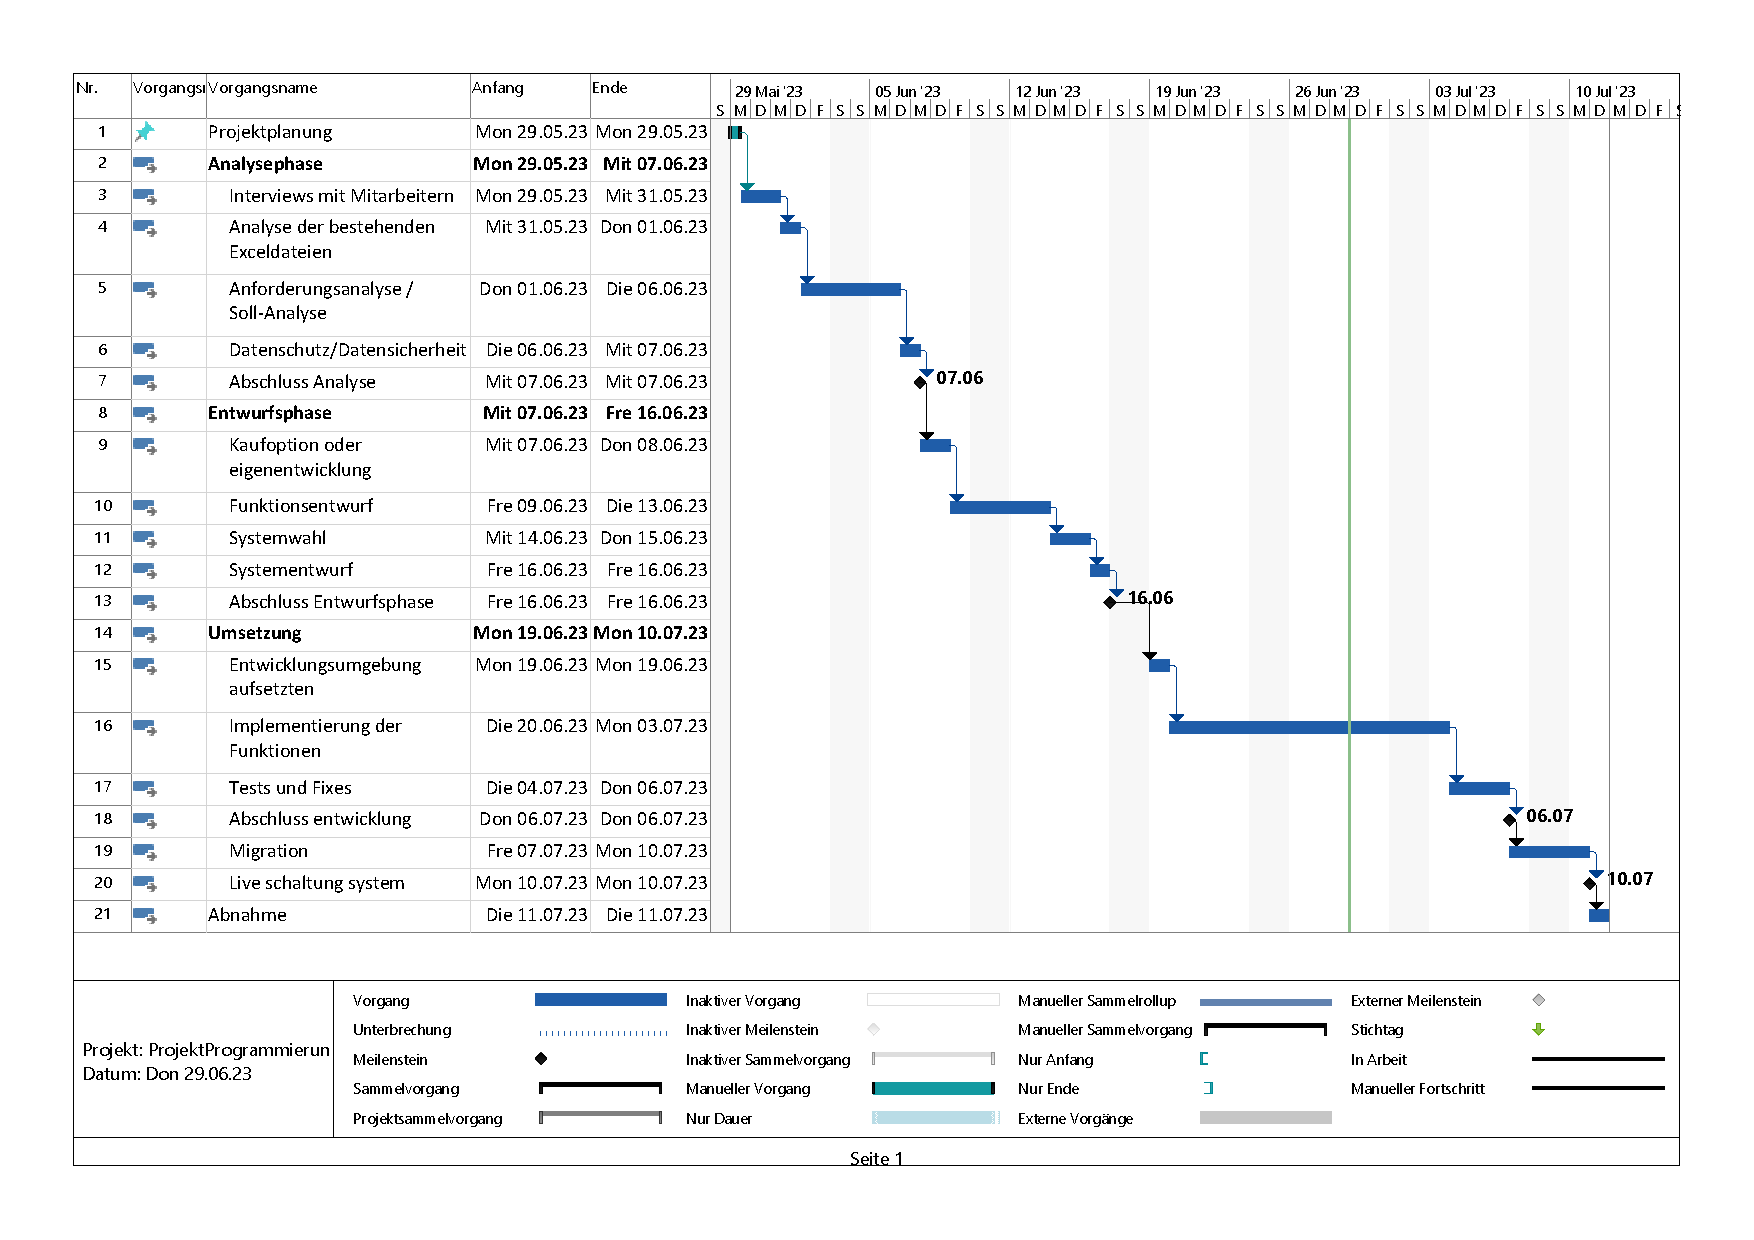
\includegraphics[angle=90, page=1,height=0.90\textheight, keepaspectratio]{anhang/abb/ProjektProgrammierungZeitplan.pdf}
    \caption[Ganttdiagramm]{Gantt}
    \label{abb:Gantt}
\end{figure}

\begin{figure}[htb]
    \centering
    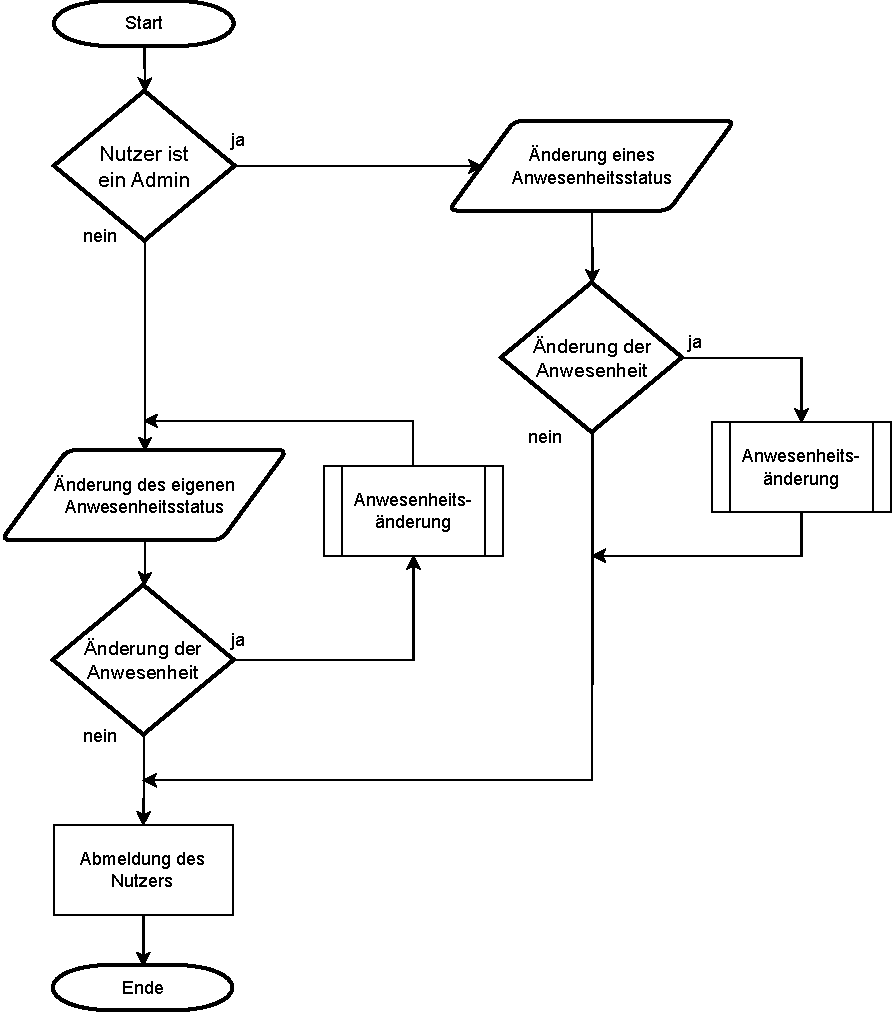
\includegraphics[width=0.9\textwidth,angle=0]{anhang/abb/PAP_Kurz.pdf}
    \caption[Programmablaufplan]{PAP änderungsvorgang von Anwesenheiten}
    \label{abb:PAP}
\end{figure}

\begin{figure}[htb]
    \centering
    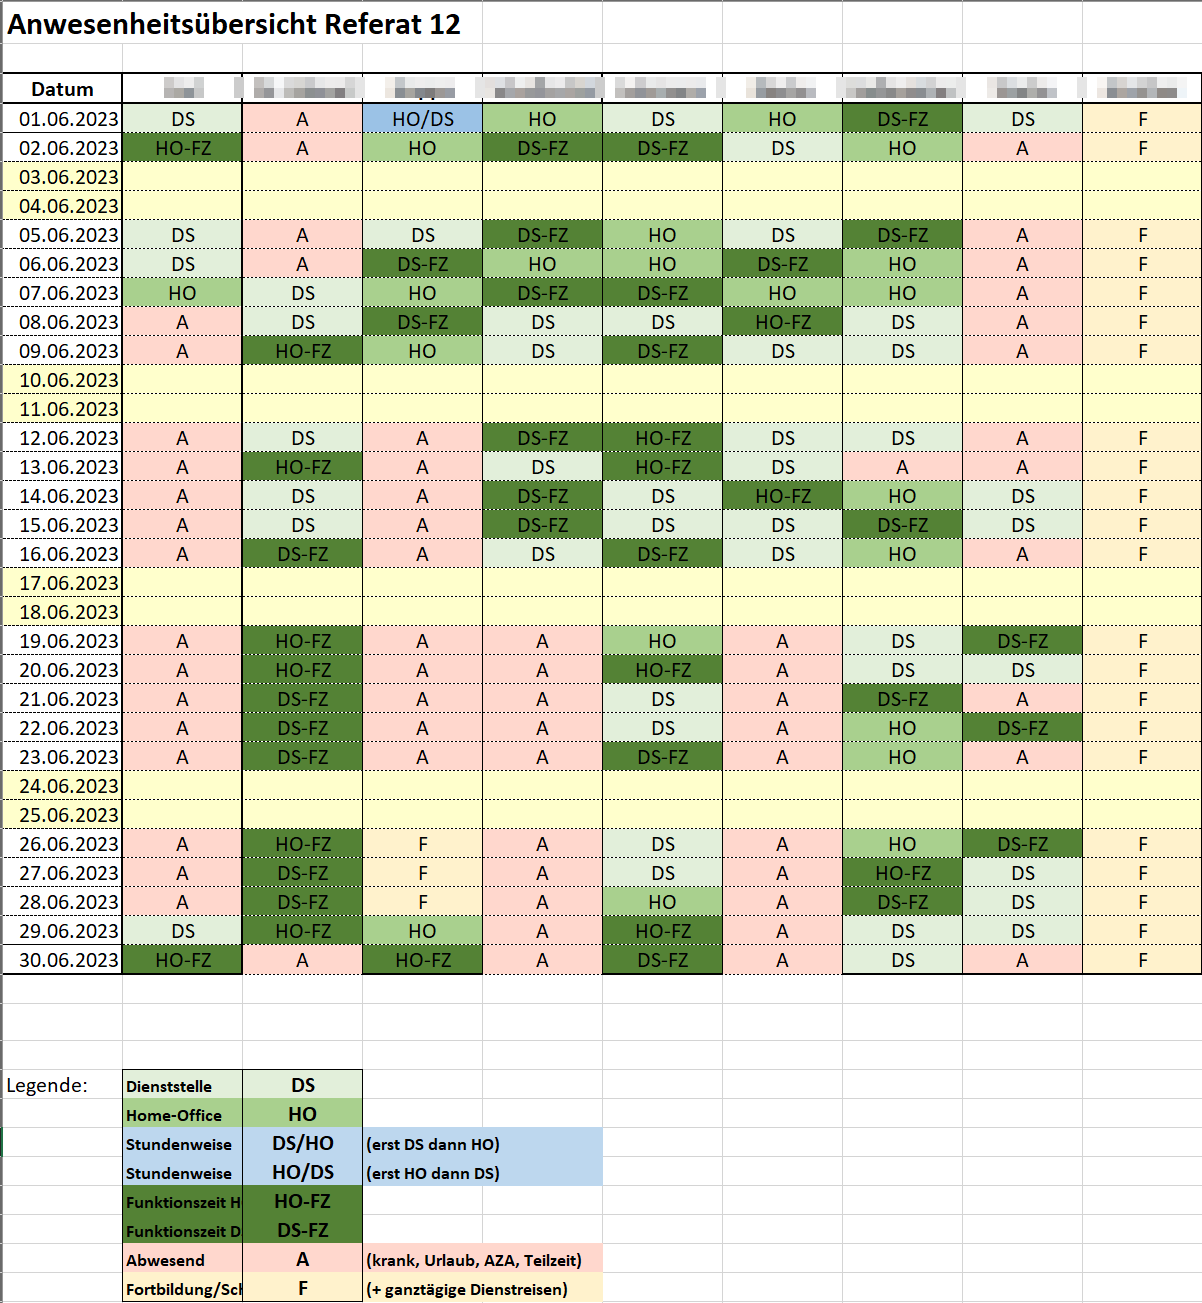
\includegraphics[width=0.9\textwidth,angle=0]{anhang/abb/Tabelle.png}
    \caption[Referenztabelle]{Referenztabelle}
    \label{abb:Ausgangstabelle}
\end{figure}

\begin{figure}[htb]
    \centering
    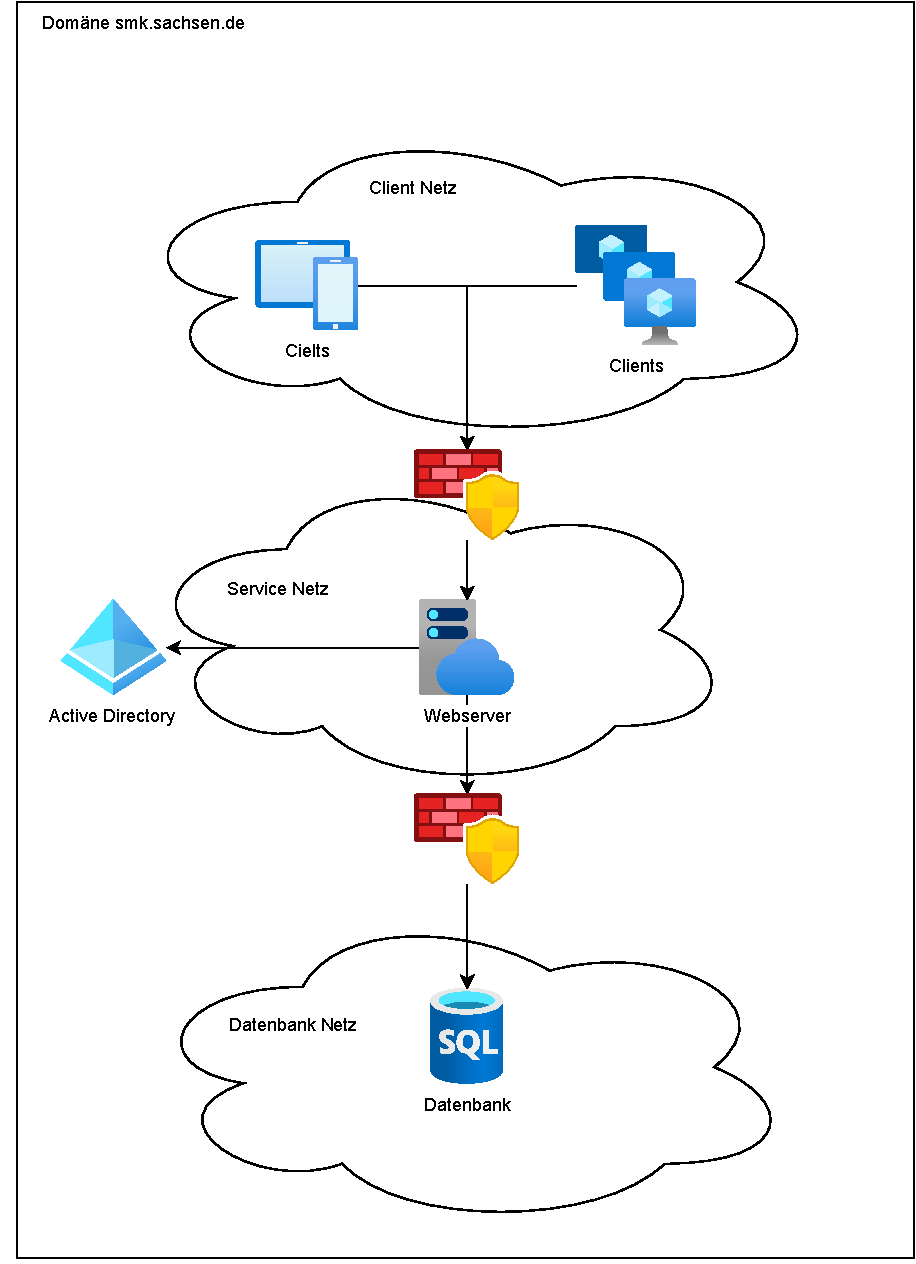
\includegraphics[width=0.9\textwidth,angle=0]{anhang/abb/Systemarchitektur.pdf}
    \caption[Skizze der Systemarchitektur]{Systemarchitektur}
    \label{abb:Systemarchitektur}
\end{figure}

\begin{figure}[htb]
    \centering
    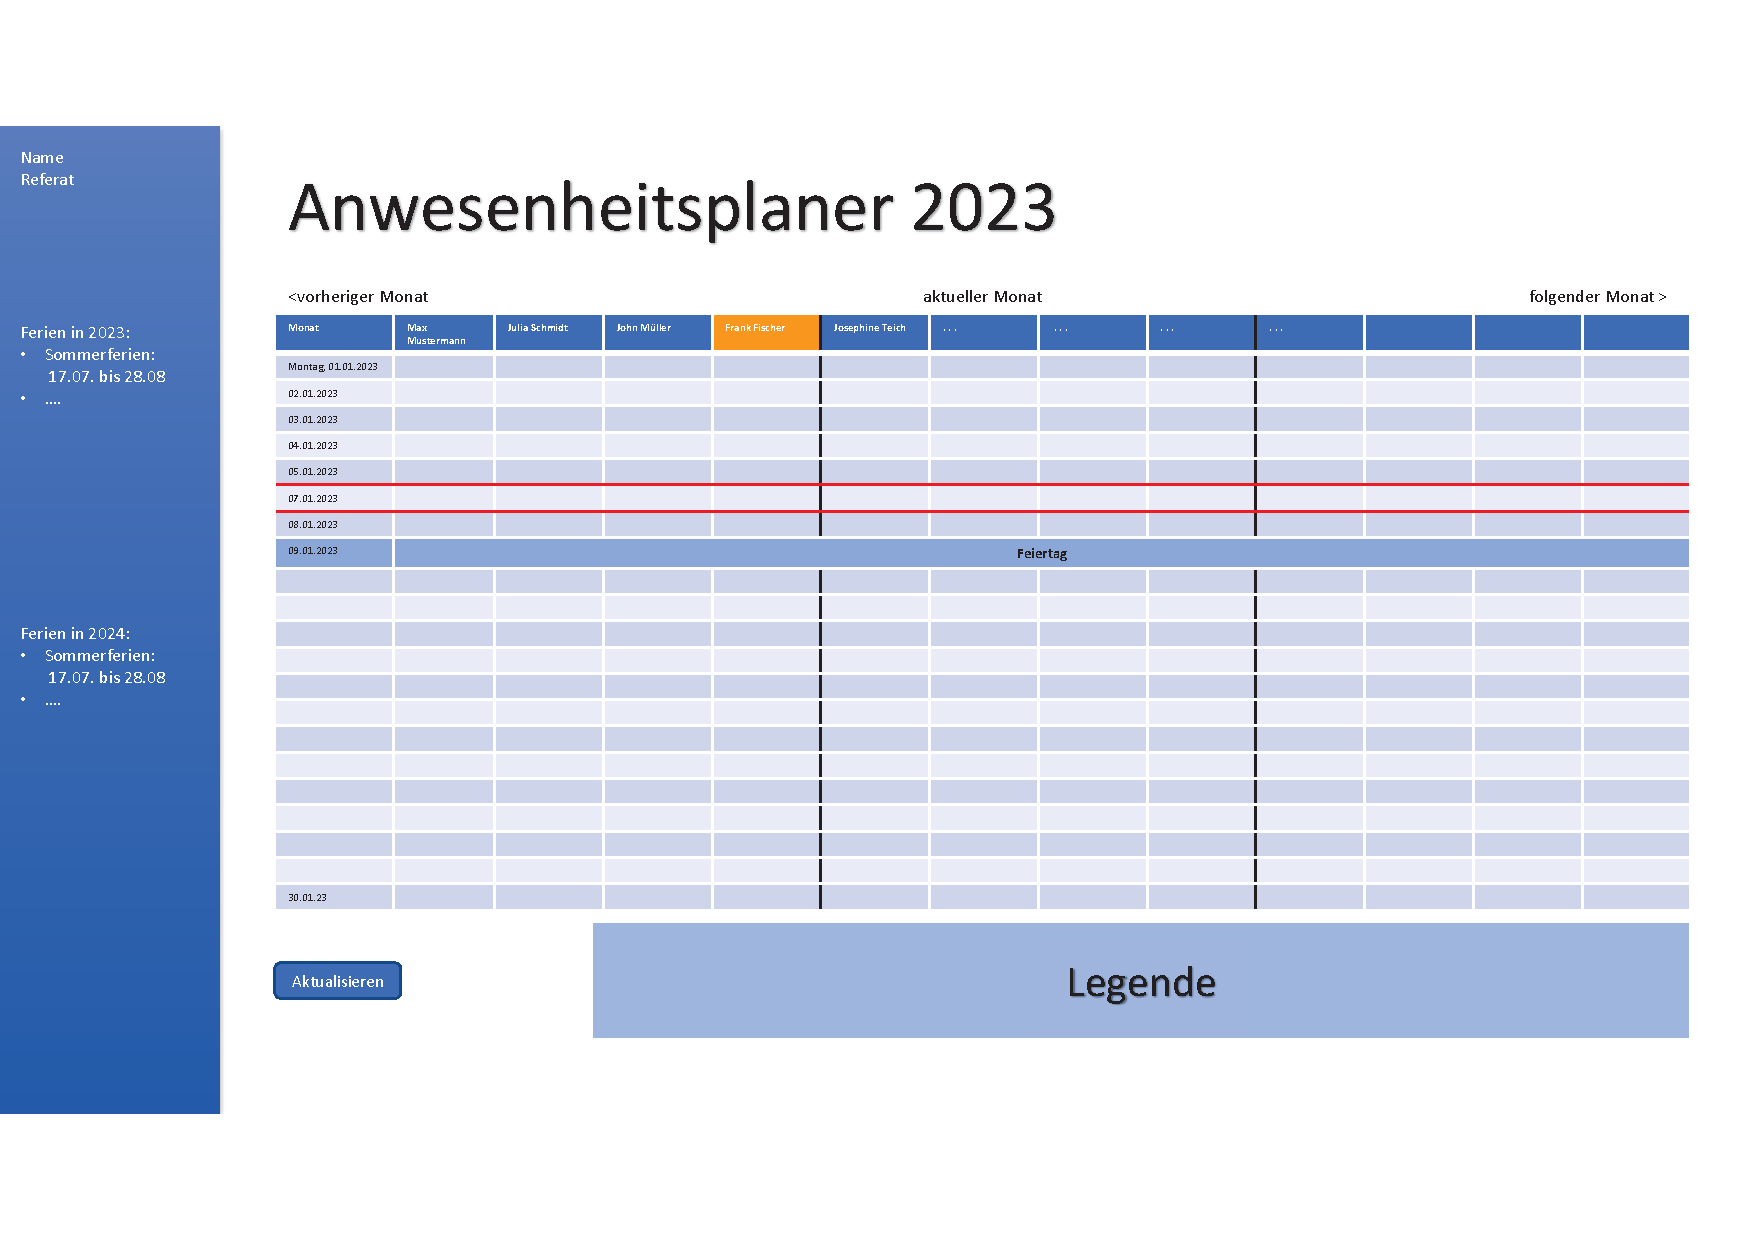
\includegraphics[angle=90, page=1,height=0.90\textheight, keepaspectratio]{anhang/abb/gui.pdf}
    \caption[GUI Entwurf]{GUI Entwurf}
    \label{abb:GUIEntwurf}
\end{figure}

\begin{figure}[htb]
    \centering
    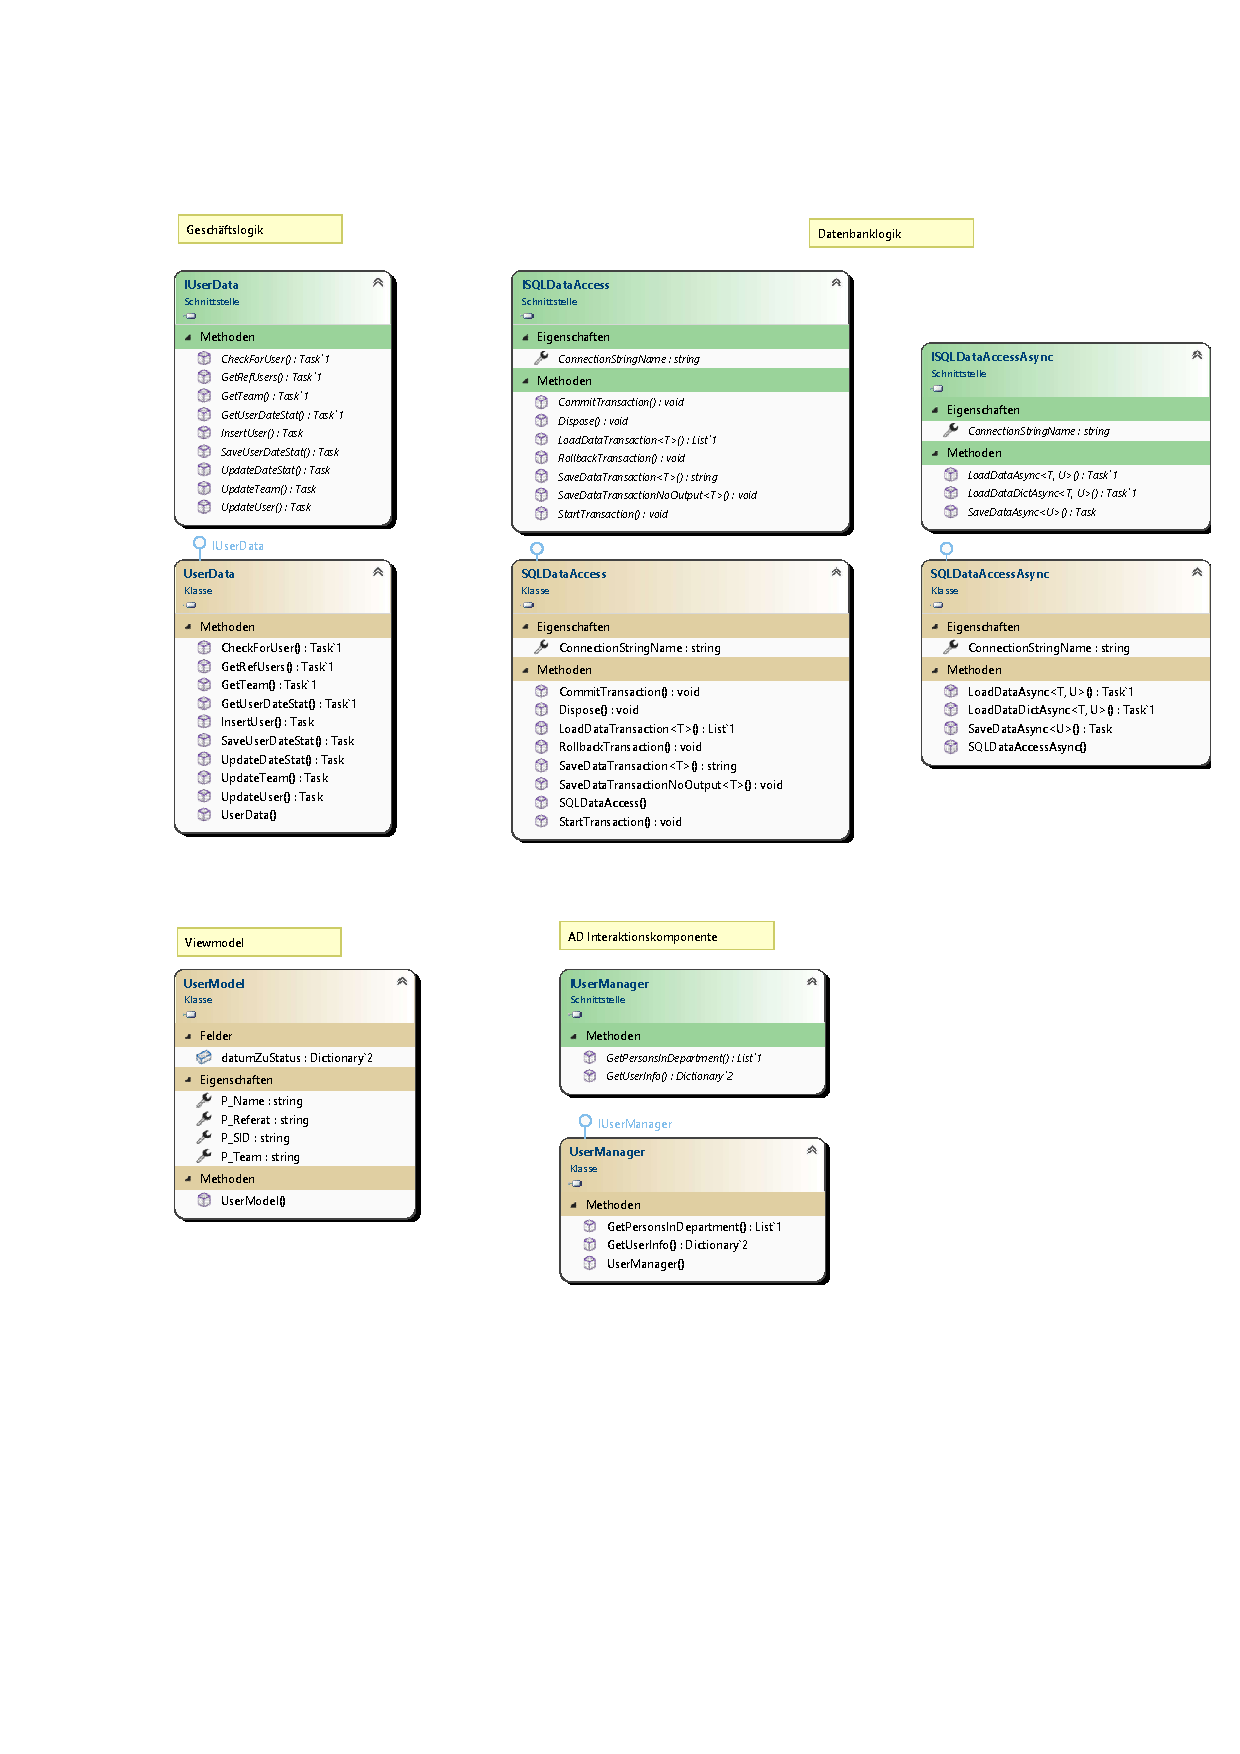
\includegraphics[width=1\textwidth,angle=0]{anhang/abb/Klassendiagramm.pdf}
    \caption[Klassendiagramm]{Klassendiagramm}
    \label{abb:Klassendiagramm}
\end{figure}

\begin{figure}[htb]
    \centering
    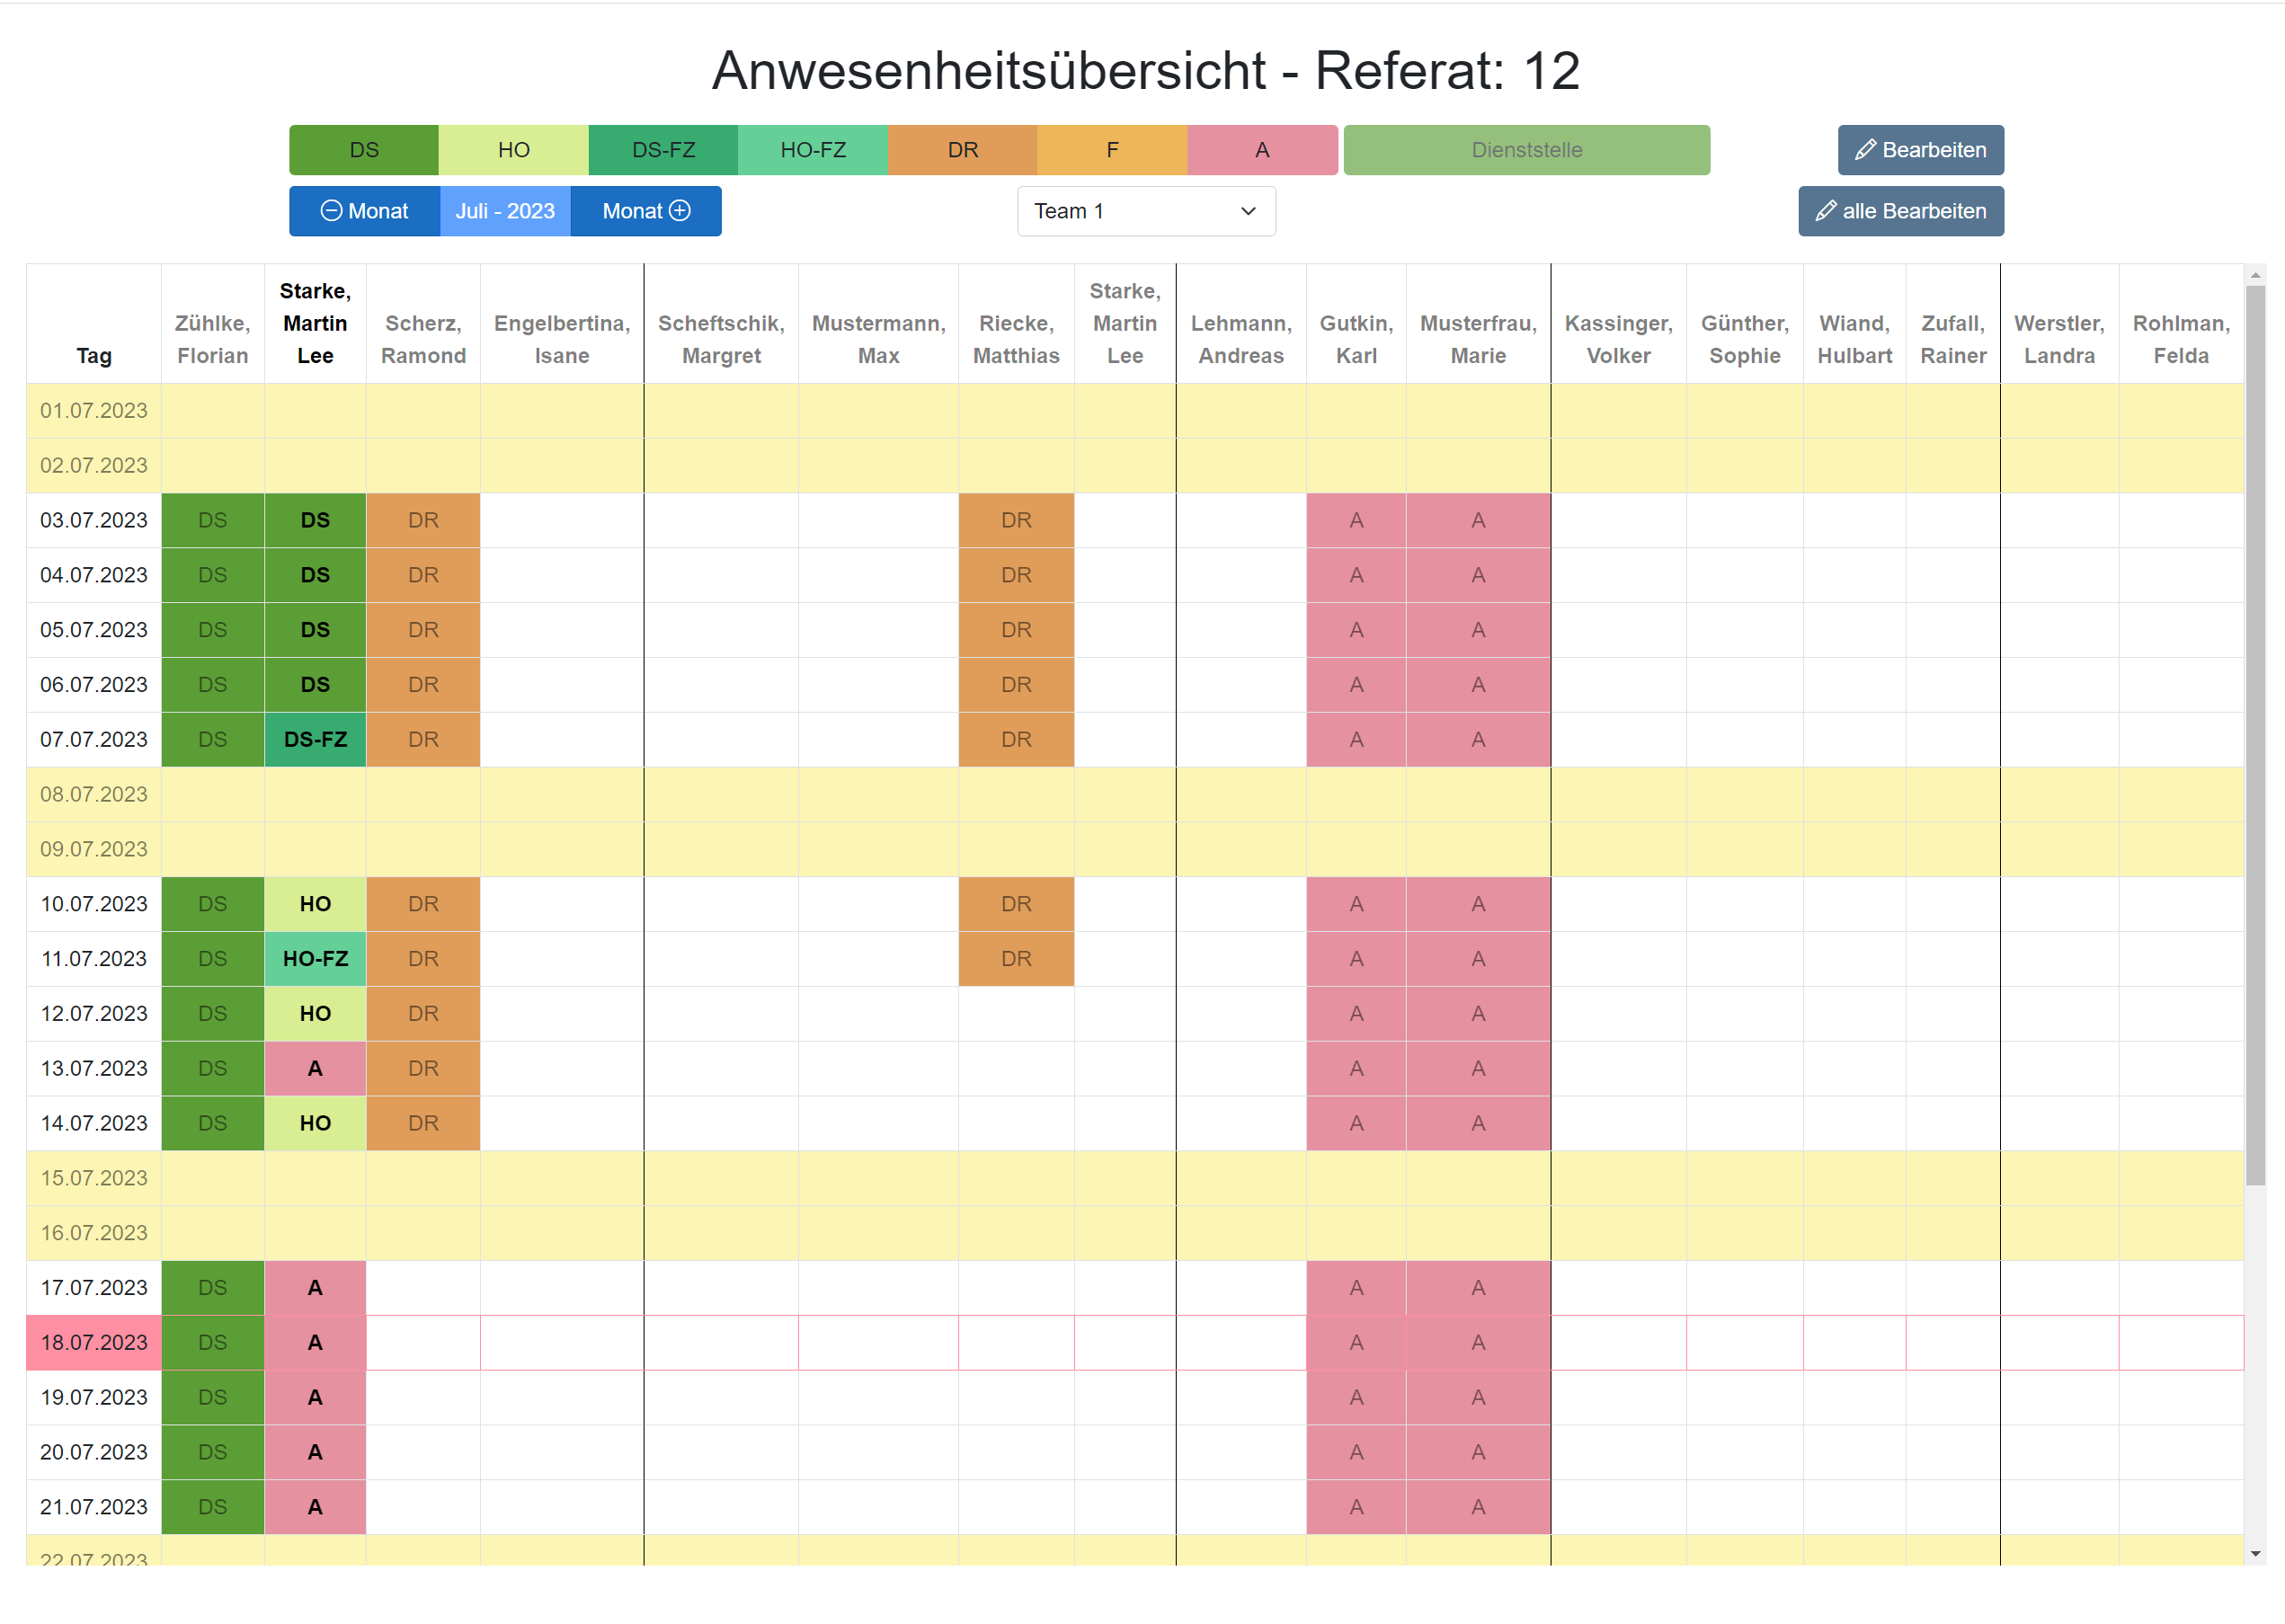
\includegraphics[angle=90, page=1,height=0.90\textheight, keepaspectratio]{abb/Prototyp_GUI.png}
    \caption[Benutzeroberfläche des Prototyps]{Prototyp}
    \label{abb:Prototyp}
\end{figure}

\section{Programmcode}
\label{Programmcode}
Der Programmcode ist Verfügbar unter:\\
https://sidas24.extranet.sachsen.de/public/download-shares/4QizdzmeHzoXnZSjQT3XTCx5GmJmElp2

